\documentclass[dvipsnames,tikz]{standalone}
\usepackage{amsmath}
\usepackage{xcolor}
\usepackage{tikz}
\usetikzlibrary{calc}
\usetikzlibrary{decorations.pathreplacing,calligraphy,3d}
\usetikzlibrary{positioning}

\tikzset{main/.style={draw=black, circle, color=black}}

\begin{document}
	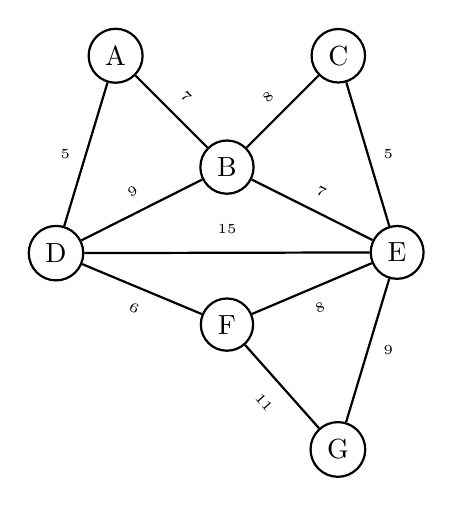
\begin{tikzpicture}[node distance={20mm}, thick] 
		\node[main] (A) {A}; 
		\node[main] (B) [below right of=A] {B};
		\node[main] (C) [above right of=B] {C};
		\node[main] (D) [below left= 2cm and 0.25cm of A] {D};
		\node[main] (E) [below right= 2cm and 0.25cm of C] {E};
		\node[main] (F) [below of=B] {F};
		\node[main] (G) [below left= 2cm and 0.25cm of E] {G};
		
		\begin{scope}[font=\tiny]
			\draw[main] (A) -- node[midway, above, sloped] {7} (B);
			\draw[main] (B) -- node[midway, above, sloped] {8} (C);
			\draw[main] (A) -- node[midway, left] {5} (D);
			\draw[main] (C) -- node[midway, right] {5} (E);
			\draw[main] (D) -- node[midway, above, sloped] {9} (B);
			\draw[main] (B) -- node[midway, above, sloped] {7} (E);
			\draw[main] (D) -- node[midway, above] {15} (E);
			\draw[main] (D) -- node[midway, below, sloped] {6} (F);
			\draw[main] (F) -- node[midway, below, sloped] {11} (G);
			\draw[main] (F) -- node[midway, below, sloped] {8} (E);
			\draw[main] (E) -- node[midway, right] {9} (G);
		\end{scope}
	\end{tikzpicture} 
	
	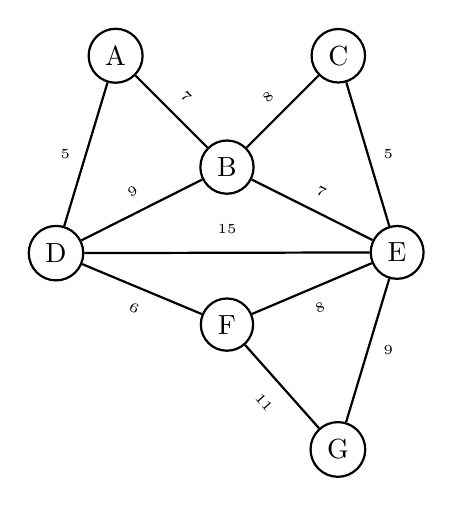
\begin{tikzpicture}[node distance={20mm}, thick] 
		\node[main] (A) {A}; 
		\node[main] (B) [below right of=A] {B};
		\node[main] (C) [above right of=B] {C};
		\node[main] (D) [below left= 2cm and 0.25cm of A] {D};
		\node[main] (E) [below right= 2cm and 0.25cm of C] {E};
		\node[main] (F) [below of=B] {F};
		\node[main] (G) [below left= 2cm and 0.25cm of E] {G};
		
		\begin{scope}[font=\tiny]
			\draw[main] (A) -- node[midway, above, sloped] {7} (B);
			\draw[main] (B) -- node[midway, above, sloped] {8} (C);
			\draw[main] (A) -- node[midway, left] {5} (D);
			\draw[main] (C) -- node[midway, right] {5} (E);
			\draw[main] (D) -- node[midway, above, sloped] {9} (B);
			\draw[main] (B) -- node[midway, above, sloped] {7} (E);
			\draw[main] (D) -- node[midway, above] {15} (E);
			\draw[main] (D) -- node[midway, below, sloped] {6} (F);
			\draw[main] (F) -- node[midway, below, sloped] {11} (G);
			\draw[main] (F) -- node[midway, below, sloped] {8} (E);
			\draw[main] (E) -- node[midway, right] {9} (G);
		\end{scope}
	\end{tikzpicture} 
	
	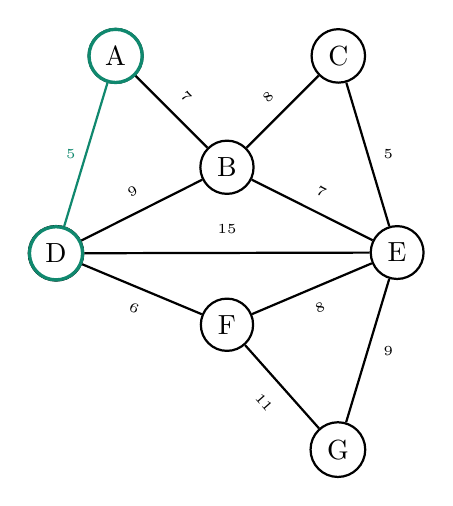
\begin{tikzpicture}[node distance={20mm}, thick] 
		\node[main] (A) {A}; 
		\node[main] (B) [below right of=A] {B};
		\node[main] (C) [above right of=B] {C};
		\node[main] (D) [below left= 2cm and 0.25cm of A] {D};
		\node[main] (E) [below right= 2cm and 0.25cm of C] {E};
		\node[main] (F) [below of=B] {F};
		\node[main] (G) [below left= 2cm and 0.25cm of E] {G};
		
		\begin{scope}[font=\tiny]
			\draw[main] (A) -- node[midway, above, sloped] {7} (B);
			\draw[main] (B) -- node[midway, above, sloped] {8} (C);
			\draw[PineGreen] (A) -- node[midway, left] {5} (D);
			\draw[main] (C) -- node[midway, right] {5} (E);
			\draw[main] (D) -- node[midway, above, sloped] {9} (B);
			\draw[main] (B) -- node[midway, above, sloped] {7} (E);
			\draw[main] (D) -- node[midway, above] {15} (E);
			\draw[main] (D) -- node[midway, below, sloped] {6} (F);
			\draw[main] (F) -- node[midway, below, sloped] {11} (G);
			\draw[main] (F) -- node[midway, below, sloped] {8} (E);
			\draw[main] (E) -- node[midway, right] {9} (G);
		\end{scope}
		
		\draw[PineGreen, very thick] (D) circle (3.375mm);
		\draw[PineGreen, very thick] (A) circle (3.375mm);
	\end{tikzpicture} 
	
	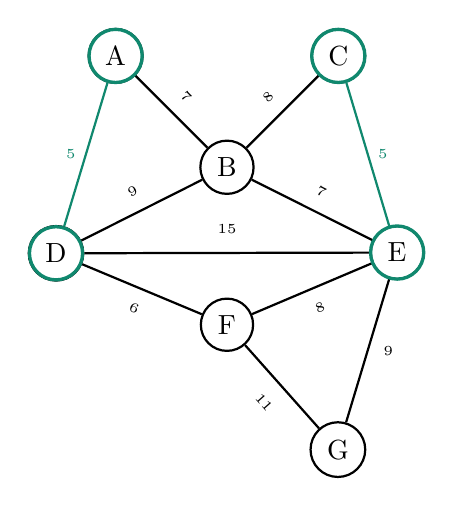
\begin{tikzpicture}[node distance={20mm}, thick] 
		\node[main] (A) {A}; 
		\node[main] (B) [below right of=A] {B};
		\node[main] (C) [above right of=B] {C};
		\node[main] (D) [below left= 2cm and 0.25cm of A] {D};
		\node[main] (E) [below right= 2cm and 0.25cm of C] {E};
		\node[main] (F) [below of=B] {F};
		\node[main] (G) [below left= 2cm and 0.25cm of E] {G};
		
		\begin{scope}[font=\tiny]
			\draw[main] (A) -- node[midway, above, sloped] {7} (B);
			\draw[main] (B) -- node[midway, above, sloped] {8} (C);
			\draw[PineGreen] (A) -- node[midway, left] {5} (D);
			\draw[PineGreen] (C) -- node[midway, right] {5} (E);
			\draw[main] (D) -- node[midway, above, sloped] {9} (B);
			\draw[main] (B) -- node[midway, above, sloped] {7} (E);
			\draw[main] (D) -- node[midway, above] {15} (E);
			\draw[main] (D) -- node[midway, below, sloped] {6} (F);
			\draw[main] (F) -- node[midway, below, sloped] {11} (G);
			\draw[main] (F) -- node[midway, below, sloped] {8} (E);
			\draw[main] (E) -- node[midway, right] {9} (G);
		\end{scope}
		
		\draw[PineGreen, very thick] (D) circle (3.375mm);
		\draw[PineGreen, very thick] (A) circle (3.375mm);
		\draw[PineGreen, very thick] (C) circle (3.375mm);
		\draw[PineGreen, very thick] (E) circle (3.375mm);
	\end{tikzpicture}
	
	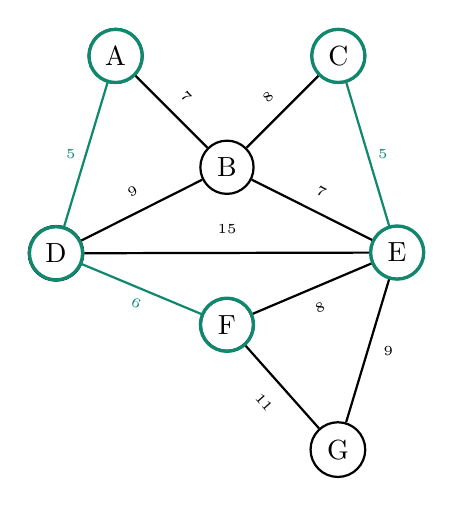
\begin{tikzpicture}[node distance={20mm}, thick] 
		\node[main] (A) {A}; 
		\node[main] (B) [below right of=A] {B};
		\node[main] (C) [above right of=B] {C};
		\node[main] (D) [below left= 2cm and 0.25cm of A] {D};
		\node[main] (E) [below right= 2cm and 0.25cm of C] {E};
		\node[main] (F) [below of=B] {F};
		\node[main] (G) [below left= 2cm and 0.25cm of E] {G};
		
		\begin{scope}[font=\tiny]
			\draw[main] (A) -- node[midway, above, sloped] {7} (B);
			\draw[main] (B) -- node[midway, above, sloped] {8} (C);
			\draw[PineGreen] (A) -- node[midway, left] {5} (D);
			\draw[PineGreen] (C) -- node[midway, right] {5} (E);
			\draw[main] (D) -- node[midway, above, sloped] {9} (B);
			\draw[main] (B) -- node[midway, above, sloped] {7} (E);
			\draw[main] (D) -- node[midway, above] {15} (E);
			\draw[PineGreen] (D) -- node[midway, below, sloped] {6} (F);
			\draw[main] (F) -- node[midway, below, sloped] {11} (G);
			\draw[main] (F) -- node[midway, below, sloped] {8} (E);
			\draw[main] (E) -- node[midway, right] {9} (G);
		\end{scope}
		
		\draw[PineGreen, very thick] (D) circle (3.375mm);
		\draw[PineGreen, very thick] (A) circle (3.375mm);
		\draw[PineGreen, very thick] (C) circle (3.375mm);
		\draw[PineGreen, very thick] (E) circle (3.375mm);
		\draw[PineGreen, very thick] (F) circle (3.375mm);
	\end{tikzpicture}
	
	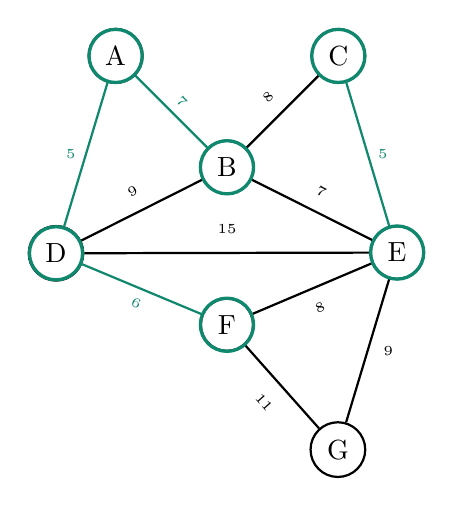
\begin{tikzpicture}[node distance={20mm}, thick] 
		\node[main] (A) {A}; 
		\node[main] (B) [below right of=A] {B};
		\node[main] (C) [above right of=B] {C};
		\node[main] (D) [below left= 2cm and 0.25cm of A] {D};
		\node[main] (E) [below right= 2cm and 0.25cm of C] {E};
		\node[main] (F) [below of=B] {F};
		\node[main] (G) [below left= 2cm and 0.25cm of E] {G};
		
		\begin{scope}[font=\tiny]
			\draw[PineGreen] (A) -- node[midway, above, sloped] {7} (B);
			\draw[main] (B) -- node[midway, above, sloped] {8} (C);
			\draw[PineGreen] (A) -- node[midway, left] {5} (D);
			\draw[PineGreen] (C) -- node[midway, right] {5} (E);
			\draw[main] (D) -- node[midway, above, sloped] {9} (B);
			\draw[main] (B) -- node[midway, above, sloped] {7} (E);
			\draw[main] (D) -- node[midway, above] {15} (E);
			\draw[PineGreen] (D) -- node[midway, below, sloped] {6} (F);
			\draw[main] (F) -- node[midway, below, sloped] {11} (G);
			\draw[main] (F) -- node[midway, below, sloped] {8} (E);
			\draw[main] (E) -- node[midway, right] {9} (G);
		\end{scope}
		
		\draw[PineGreen, very thick] (D) circle (3.375mm);
		\draw[PineGreen, very thick] (A) circle (3.375mm);
		\draw[PineGreen, very thick] (C) circle (3.375mm);
		\draw[PineGreen, very thick] (E) circle (3.375mm);
		\draw[PineGreen, very thick] (F) circle (3.375mm);
		\draw[PineGreen, very thick] (B) circle (3.375mm);
	\end{tikzpicture}
	
	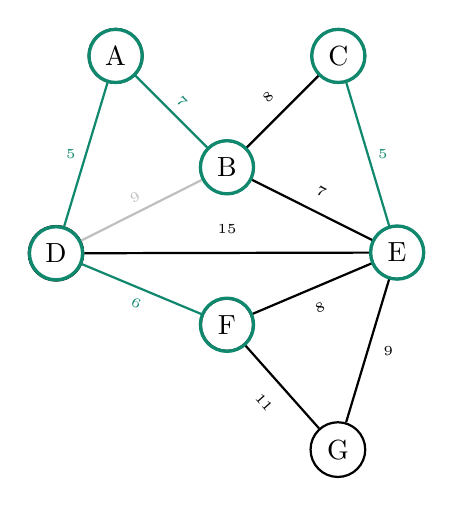
\begin{tikzpicture}[node distance={20mm}, thick] 
		\node[main] (A) {A}; 
		\node[main] (B) [below right of=A] {B};
		\node[main] (C) [above right of=B] {C};
		\node[main] (D) [below left= 2cm and 0.25cm of A] {D};
		\node[main] (E) [below right= 2cm and 0.25cm of C] {E};
		\node[main] (F) [below of=B] {F};
		\node[main] (G) [below left= 2cm and 0.25cm of E] {G};
		
		\begin{scope}[font=\tiny]
			\draw[PineGreen] (A) -- node[midway, above, sloped] {7} (B);
			\draw[main] (B) -- node[midway, above, sloped] {8} (C);
			\draw[PineGreen] (A) -- node[midway, left] {5} (D);
			\draw[PineGreen] (C) -- node[midway, right] {5} (E);
			\draw[lightgray] (D) -- node[midway, above, sloped] {9} (B);
			\draw[main] (B) -- node[midway, above, sloped] {7} (E);
			\draw[main] (D) -- node[midway, above] {15} (E);
			\draw[PineGreen] (D) -- node[midway, below, sloped] {6} (F);
			\draw[main] (F) -- node[midway, below, sloped] {11} (G);
			\draw[main] (F) -- node[midway, below, sloped] {8} (E);
			\draw[main] (E) -- node[midway, right] {9} (G);
		\end{scope}
		
		\draw[PineGreen, very thick] (D) circle (3.375mm);
		\draw[PineGreen, very thick] (A) circle (3.375mm);
		\draw[PineGreen, very thick] (C) circle (3.375mm);
		\draw[PineGreen, very thick] (E) circle (3.375mm);
		\draw[PineGreen, very thick] (F) circle (3.375mm);
		\draw[PineGreen, very thick] (B) circle (3.375mm);
	\end{tikzpicture}
	
	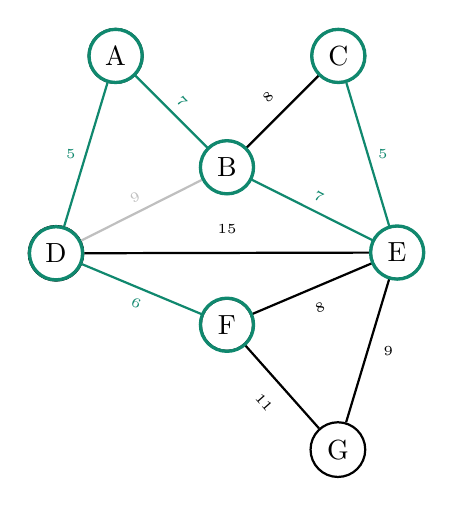
\begin{tikzpicture}[node distance={20mm}, thick] 
		\node[main] (A) {A}; 
		\node[main] (B) [below right of=A] {B};
		\node[main] (C) [above right of=B] {C};
		\node[main] (D) [below left= 2cm and 0.25cm of A] {D};
		\node[main] (E) [below right= 2cm and 0.25cm of C] {E};
		\node[main] (F) [below of=B] {F};
		\node[main] (G) [below left= 2cm and 0.25cm of E] {G};
		
		\begin{scope}[font=\tiny]
			\draw[PineGreen] (A) -- node[midway, above, sloped] {7} (B);
			\draw[main] (B) -- node[midway, above, sloped] {8} (C);
			\draw[PineGreen] (A) -- node[midway, left] {5} (D);
			\draw[PineGreen] (C) -- node[midway, right] {5} (E);
			\draw[lightgray] (D) -- node[midway, above, sloped] {9} (B);
			\draw[PineGreen] (B) -- node[midway, above, sloped] {7} (E);
			\draw[main] (D) -- node[midway, above] {15} (E);
			\draw[PineGreen] (D) -- node[midway, below, sloped] {6} (F);
			\draw[main] (F) -- node[midway, below, sloped] {11} (G);
			\draw[main] (F) -- node[midway, below, sloped] {8} (E);
			\draw[main] (E) -- node[midway, right] {9} (G);
		\end{scope}
		
		\draw[PineGreen, very thick] (D) circle (3.375mm);
		\draw[PineGreen, very thick] (A) circle (3.375mm);
		\draw[PineGreen, very thick] (C) circle (3.375mm);
		\draw[PineGreen, very thick] (E) circle (3.375mm);
		\draw[PineGreen, very thick] (F) circle (3.375mm);
		\draw[PineGreen, very thick] (B) circle (3.375mm);
	\end{tikzpicture}
	
	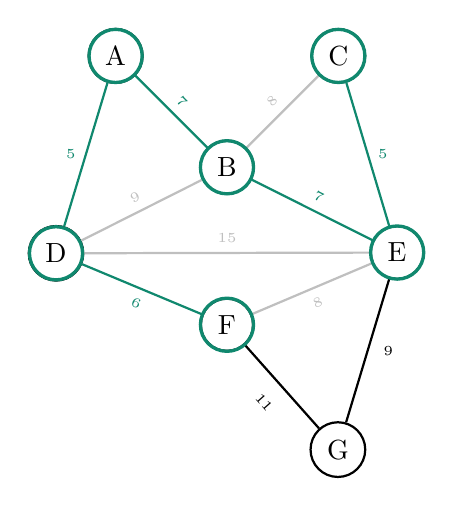
\begin{tikzpicture}[node distance={20mm}, thick] 
		\node[main] (A) {A}; 
		\node[main] (B) [below right of=A] {B};
		\node[main] (C) [above right of=B] {C};
		\node[main] (D) [below left= 2cm and 0.25cm of A] {D};
		\node[main] (E) [below right= 2cm and 0.25cm of C] {E};
		\node[main] (F) [below of=B] {F};
		\node[main] (G) [below left= 2cm and 0.25cm of E] {G};
		
		\begin{scope}[font=\tiny]
			\draw[PineGreen] (A) -- node[midway, above, sloped] {7} (B);
			\draw[lightgray] (B) -- node[midway, above, sloped] {8} (C);
			\draw[PineGreen] (A) -- node[midway, left] {5} (D);
			\draw[PineGreen] (C) -- node[midway, right] {5} (E);
			\draw[lightgray] (D) -- node[midway, above, sloped] {9} (B);
			\draw[PineGreen] (B) -- node[midway, above, sloped] {7} (E);
			\draw[lightgray] (D) -- node[midway, above] {15} (E);
			\draw[PineGreen] (D) -- node[midway, below, sloped] {6} (F);
			\draw[main] (F) -- node[midway, below, sloped] {11} (G);
			\draw[lightgray] (F) -- node[midway, below, sloped] {8} (E);
			\draw[main] (E) -- node[midway, right] {9} (G);
		\end{scope}
		
		\draw[PineGreen, very thick] (D) circle (3.375mm);
		\draw[PineGreen, very thick] (A) circle (3.375mm);
		\draw[PineGreen, very thick] (C) circle (3.375mm);
		\draw[PineGreen, very thick] (E) circle (3.375mm);
		\draw[PineGreen, very thick] (F) circle (3.375mm);
		\draw[PineGreen, very thick] (B) circle (3.375mm);
	\end{tikzpicture}
	
	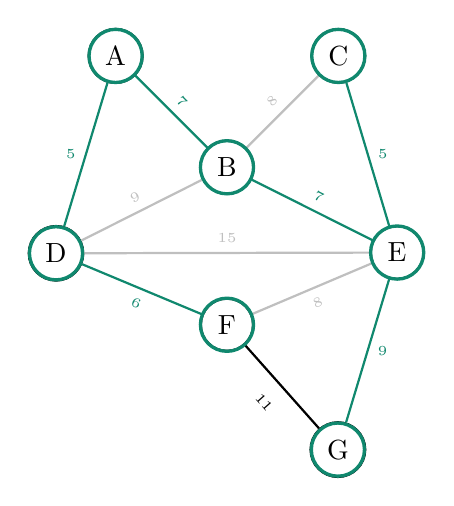
\begin{tikzpicture}[node distance={20mm}, thick] 
		\node[main] (A) {A}; 
		\node[main] (B) [below right of=A] {B};
		\node[main] (C) [above right of=B] {C};
		\node[main] (D) [below left= 2cm and 0.25cm of A] {D};
		\node[main] (E) [below right= 2cm and 0.25cm of C] {E};
		\node[main] (F) [below of=B] {F};
		\node[main] (G) [below left= 2cm and 0.25cm of E] {G};
		
		\begin{scope}[font=\tiny]
			\draw[PineGreen] (A) -- node[midway, above, sloped] {7} (B);
			\draw[lightgray] (B) -- node[midway, above, sloped] {8} (C);
			\draw[PineGreen] (A) -- node[midway, left] {5} (D);
			\draw[PineGreen] (C) -- node[midway, right] {5} (E);
			\draw[lightgray] (D) -- node[midway, above, sloped] {9} (B);
			\draw[PineGreen] (B) -- node[midway, above, sloped] {7} (E);
			\draw[lightgray] (D) -- node[midway, above] {15} (E);
			\draw[PineGreen] (D) -- node[midway, below, sloped] {6} (F);
			\draw[main] (F) -- node[midway, below, sloped] {11} (G);
			\draw[lightgray] (F) -- node[midway, below, sloped] {8} (E);
			\draw[PineGreen] (E) -- node[midway, right] {9} (G);
		\end{scope}
		
		\draw[PineGreen, very thick] (D) circle (3.375mm);
		\draw[PineGreen, very thick] (A) circle (3.375mm);
		\draw[PineGreen, very thick] (C) circle (3.375mm);
		\draw[PineGreen, very thick] (E) circle (3.375mm);
		\draw[PineGreen, very thick] (F) circle (3.375mm);
		\draw[PineGreen, very thick] (B) circle (3.375mm);
		\draw[PineGreen, very thick] (G) circle (3.375mm);
	\end{tikzpicture}
	
	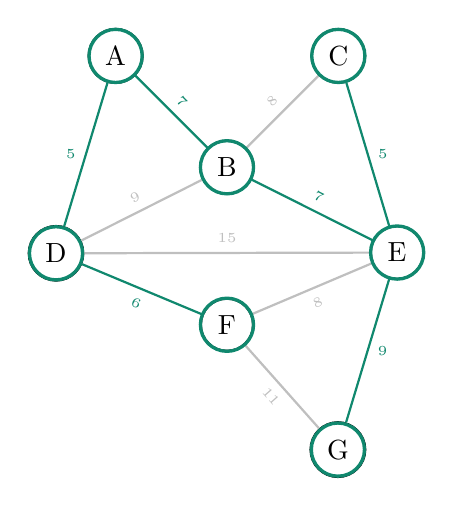
\begin{tikzpicture}[node distance={20mm}, thick] 
		\node[main] (A) {A}; 
		\node[main] (B) [below right of=A] {B};
		\node[main] (C) [above right of=B] {C};
		\node[main] (D) [below left= 2cm and 0.25cm of A] {D};
		\node[main] (E) [below right= 2cm and 0.25cm of C] {E};
		\node[main] (F) [below of=B] {F};
		\node[main] (G) [below left= 2cm and 0.25cm of E] {G};
		
		\begin{scope}[font=\tiny]
			\draw[PineGreen] (A) -- node[midway, above, sloped] {7} (B);
			\draw[lightgray] (B) -- node[midway, above, sloped] {8} (C);
			\draw[PineGreen] (A) -- node[midway, left] {5} (D);
			\draw[PineGreen] (C) -- node[midway, right] {5} (E);
			\draw[lightgray] (D) -- node[midway, above, sloped] {9} (B);
			\draw[PineGreen] (B) -- node[midway, above, sloped] {7} (E);
			\draw[lightgray] (D) -- node[midway, above] {15} (E);
			\draw[PineGreen] (D) -- node[midway, below, sloped] {6} (F);
			\draw[lightgray] (F) -- node[midway, below, sloped] {11} (G);
			\draw[lightgray] (F) -- node[midway, below, sloped] {8} (E);
			\draw[PineGreen] (E) -- node[midway, right] {9} (G);
		\end{scope}
		
		\draw[PineGreen, very thick] (D) circle (3.375mm);
		\draw[PineGreen, very thick] (A) circle (3.375mm);
		\draw[PineGreen, very thick] (C) circle (3.375mm);
		\draw[PineGreen, very thick] (E) circle (3.375mm);
		\draw[PineGreen, very thick] (F) circle (3.375mm);
		\draw[PineGreen, very thick] (B) circle (3.375mm);
		\draw[PineGreen, very thick] (G) circle (3.375mm);
	\end{tikzpicture}
	
	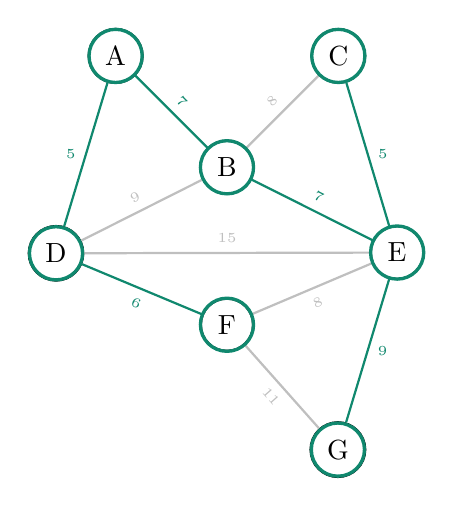
\begin{tikzpicture}[node distance={20mm}, thick] 
		\node[main] (A) {A}; 
		\node[main] (B) [below right of=A] {B};
		\node[main] (C) [above right of=B] {C};
		\node[main] (D) [below left= 2cm and 0.25cm of A] {D};
		\node[main] (E) [below right= 2cm and 0.25cm of C] {E};
		\node[main] (F) [below of=B] {F};
		\node[main] (G) [below left= 2cm and 0.25cm of E] {G};
		
		\begin{scope}[font=\tiny]
			\draw[PineGreen] (A) -- node[midway, above, sloped] {7} (B);
			\draw[lightgray] (B) -- node[midway, above, sloped] {8} (C);
			\draw[PineGreen] (A) -- node[midway, left] {5} (D);
			\draw[PineGreen] (C) -- node[midway, right] {5} (E);
			\draw[lightgray] (D) -- node[midway, above, sloped] {9} (B);
			\draw[PineGreen] (B) -- node[midway, above, sloped] {7} (E);
			\draw[lightgray] (D) -- node[midway, above] {15} (E);
			\draw[PineGreen] (D) -- node[midway, below, sloped] {6} (F);
			\draw[lightgray] (F) -- node[midway, below, sloped] {11} (G);
			\draw[lightgray] (F) -- node[midway, below, sloped] {8} (E);
			\draw[PineGreen] (E) -- node[midway, right] {9} (G);
		\end{scope}
		
		\draw[PineGreen, very thick] (D) circle (3.375mm);
		\draw[PineGreen, very thick] (A) circle (3.375mm);
		\draw[PineGreen, very thick] (C) circle (3.375mm);
		\draw[PineGreen, very thick] (E) circle (3.375mm);
		\draw[PineGreen, very thick] (F) circle (3.375mm);
		\draw[PineGreen, very thick] (B) circle (3.375mm);
		\draw[PineGreen, very thick] (G) circle (3.375mm);
	\end{tikzpicture}
	
\end{document}